\documentclass[12pt,a4paper]{article}
\usepackage[utf8]{inputenc}
\usepackage[english]{babel}
\setcounter{tocdepth}{4}
\setcounter{secnumdepth}{4}
\usepackage{xstring}
\usepackage{siunitx}
\usepackage{amsmath}
\usepackage{graphicx}
\usepackage[nottoc]{tocbibind} %Adds "References" to the table of contents
\usepackage{hyperref}
\usepackage[toc]{glossaries}
\usepackage{textcomp}
\usepackage{csvsimple}
\usepackage{pgfplotstable}
\pgfplotsset{compat=1.9}% supress warning
\usepackage{longtable}
\usepackage{xcolor,colortbl}
\usepackage{listings}
\usepackage[toc,page]{appendix}
\usepackage{fancyvrb}
\usepackage{tikz}
\usepackage{mathtools}
\usepackage{gensymb}
\usepackage{ragged2e}
\usepackage{titlesec}


% *** BIBLIOGRAPHY CONGIG *** $
\usepackage[style=nature, backend=bibtex]{biblatex}
\usepackage{csquotes}
\addbibresource{bibliography.bib}
% *************************** $

% change paragraph title fromatting
%\titleformat*{\paragraph}{\itshape\mdseries}




\lstset{ %
language=C++,           % choose the language of the code
numbers=left,           % where to put the line-numbers
numberstyle=\tiny,      % the size of the fonts that are used for the line-numbers
basicstyle=\footnotesize    % the size of the fonts that are used for the line-numbers
}

\newcommand{\mc}[2]{\multicolumn{#1}{c}{#2}}
\definecolor{Gray}{gray}{0.85}
\definecolor{LightCyan}{rgb}{0.88,1,1}

\newcolumntype{A}{>{\columncolor{Gray}}c}
\newcolumntype{B}{>{\columncolor{white}}c}

% MODIFY NUMBERING OF TABLES AND PICTURES
\usepackage{chngcntr}
\counterwithin{table}{section}
\counterwithin{figure}{section}
\counterwithin{equation}{section}
\usepackage{floatrow}
\floatsetup[table]{capposition=top}

% HEADINGS AND MARGINS 
\usepackage{geometry}
 \geometry{
 a4paper,
 left=25mm,
 right=25mm,
 top=25mm,
 bottom=25mm,
 headheight=15mm,
 footskip=15mm,
 }
 

% PAGE STYLE SECTION
\usepackage{fancyhdr}
\pagestyle{fancy}
\renewcommand\sectionmark[1]{\markboth{\thesection\ #1}{}}
\fancyhf{}
\fancyhead[C]{\bfseries\leftmark}
\fancyfoot[C]{\bfseries\thepage}
\renewcommand{\headrulewidth}{0.5pt}% suppress the header rule

% INDENTATATIONS
\usepackage{indentfirst}
\setlength{\parindent}{0.75cm}

% FONT
\usepackage{times}

% UNIVERISTY LOGO TRIGGER
\usepackage{graphicx}

% TITLES OF PARTICULAR SECTIONS
\usepackage{titlesec}

\titleformat{\section}
    {\large\bfseries\itshape}
    {\thesection}
    {1em}
    {\MakeUppercase}
\titleformat{\subsection}
    {\large\bfseries\itshape}
    {\thesubsection}
    {1em}
    {}
\titleformat{\subsubsection}
    {\large\bfseries\itshape}
    {\thesubsubsection}
    {1em}
    {}
\titleformat{\paragraph}
    {\large\bfseries}
    {\theparagraph}
    {1em}
    {}
\titleformat{\subparagraph}
    {\large\bfseries}
    {\thesubparagraph}
    {1em}
    {}
    
    
% Glossary



\begin{document}

\begin{titlepage}
    \centering
    
\includegraphics[width=7cm]{logo.jpg} % also works with 
    \vskip1cm
    {\Large
        SILESIAN UNIVERSITY OF TECHNOLOGY\\
        FACULTY OF ELECTRICAL ENGINEERING\\
        \vskip0.5cm
        Department of Power Electronics, Electrical Drives and Robotics\\
    }
    \vskip1cm
    {\bfseries\huge
    Master's thesis\\
    }
    \vskip1cm
    {\bfseries\large
    To be determined \\
    }
    \vskip2cm
    {\large
    \begin{tabular}{p{4cm} p{10cm}}
    Student: & {\bfseries\Large Igor Aleksander JANKIEWICZ}\\
    Transcript no.: & 285947\\
        &   \\
    Type of studies: & Extramural studies (MSc programme)\\
    Field of study: & Electrical Engineering\\
    Programme: & To be determined\\
        &   \\
    Supervisor: & PhD. EEng. Andrzej Latko\\
    \end{tabular}
    }
    \vskip2.5cm
    {\large
    Gliwice 2020}
\end{titlepage}
\newpage\null\thispagestyle{empty}\newpage
\tableofcontents
\newpage\null\thispagestyle{empty}\newpage

\section{Introduction}
This Master's thesis is focused on Piezoelectic Energy Harvesting in general. Apart from the explanation of the actual energy scavenging process, it also covers a design of a proper data acquisition system used for evaluation and development of piezoelectric-based generators.
\par

\subsection{Motivation}
Nowadays, electrical energy itself is taken for granted by most of the people. It may be a result of the fact that most of household appliances and daily use items require that energy to operate. Moreover, almost any of our tasks requite a proper illumination, Internet access or simply the outlet to liven any tool we might need at the moment. To conclude, it is almost impossible to imagine our life without an access to the power gird.
\par
On the other hand, it is important to keep in mind that most of electricity we utilize comes from non-renewable fuels such as coal, liquid gas or crude oil. At some point, humankind is to face a problem of insufficient deposits of these materials, therefore it tremendously important to look for alternatives. Of course, people have already taken advantage of water, wind or solar radiation, what is proven by the existence of many green power plants around the world. Unfortunately, one of the major problems faced by all of there plans is the intermittent access to the energy source. Moreover, there are many places that does not allow to use any of these well explored solutions, forcing engineers to look for new ones. This could be a reason why vibrational energy is getting more awareness over last years.
\par

Energy harvesting from vibration gives many new possibilities, especially in IoT (Internet of Things) applications, as well as in industrial environment. The second application seems particularly tempting, as in many industrial applications, there is a lot of vibration involved, what gives a wide scope for custom sensor development. Piezoelectric harvesters are relatively compact, therefore it is possible to install them in inaccessible places. Moreover, they are robust, providing that a proper enclosure is used for mechanical protection.
\par

All of mentioned factors gained author's interest, and in the event prompted to work on this subject within the confines of this thesis.
\par

\subsection{Objective of a Master's thesis}
The main goal stated by the author is to examine a potential of vibration-based energy scavenging. In order to do so, number of different aspects need a thorough investigation. Undeniably, much of the focus would be put on the energy harvester itself. Nevertheless, a proper measurement and data acquisition system is also an important aspect throughout the entire work, since it will allow confirm or deny thesis statements posed during the research. In addition, the design process of the mentioned device would allow a more in-depth analysis of the piezoelectric generator itself, since the understanding of its operation is the only way to come up with a suitable measurement system.
\par
Returning to the piezoelectric generator, the first thing to look at is the theory behind the piezoelectric effect. Then, there would be a description of the piezoelectric cantilever  and its properties. Subsequently, the complete mechanical and electrical model would be studied.
\par

Once the required theory is introduced, it is possible to focus exactly on the topic.

\section{Concept of Energy Harvesting}
Energy Harvesting is a process of using ambient energy by converting it into a usable form, i.e. electricity or heat. It is important to point out that energy harvesting has been around for quite a long time, since solar panels, wind turbines and water turbines are in constant use for a few decades, providing people with environmentally clean energy \cite{EnHv1}.
\par

There are some important issues related to any energy source that could be potentially used for harvesting. First of all, it is crucial to evaluate intensity and availability of that source. Subsequently, one should find out a cost-effectiveness of the solution as well as the influence of the harvesting process on the primary energy source \cite{EnHv1}.
\par

Vibration-based Energy Harvesting incorporates a number of different fields of study, i.e. material science, mechanics or electrical engineering, just to name a few. Last sentence implies that the analysis of a piezoelectric generator itself is not a straightforward process. The electromechanical response of this device relies thoroughly on the source of ambient energy \cite{EnHv2}.
\par

The concept of piezoelectric energy harvesting is strongly related to the improvement of electronics manufacturing technologies. Due to fact that most of devices are becoming more energy efficient, it allows to seek for potentially useful energy in solutions that have been neglected before. This perfectly applies to vibrational energy \cite{low_freq}. 

\subsection{Piezoelectric material utilized in harvesters}
Currently, the most popular material utilized in harvesters is so called PZT (lead zirconate titanate). It was developed at the Tokyo Institute of Technology in the 1950s \cite{EnHv2}. Nowadays, it can be found in a few different flavours, what would be described more precisely later. This material is a polymer composite, which is very brittle and prone to crack when overstressed\cite{cmos}.
\par

As described in the previous paragraph, PZT has a number of different types that vary with electrical and electromechanical properties. The simplest division includes hard and soft types - PZH-5H and PZH-5A, respectively. Soft piezoceramics are more susceptible to changes caused by the stress. This is one of the aspects why PZH-5H is the most common choice for piezoelectric equipment. On the other hand, one of the biggest manufacturers of harvesters \cite{PPA} is mentioning that PZH-5A is more temperature stable. Nevertheless, PZH-5H remains the best choice in terms of performance versus price. 
\par

Properties of piezoelectic materials strongly depend on the direction of the stres and orientation of the polarization \cite{EnHv1}. It is characterized by the constants listed in the Table 

\begin{figure}[ht!]
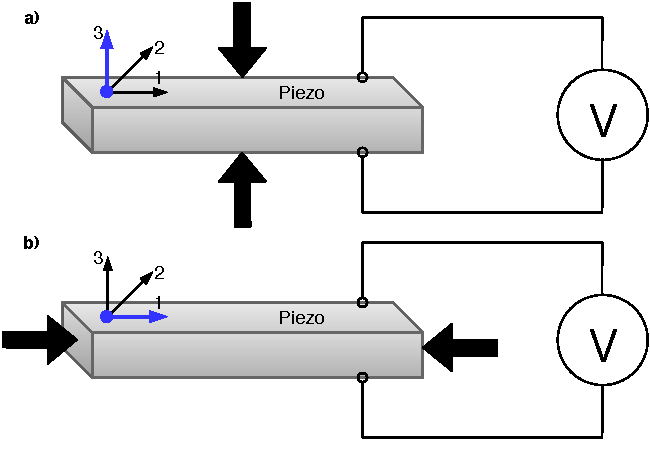
\includegraphics[scale=1]{piezo_operation_modes.pdf}
\caption{Operation modes of the piezoelectric element}
\label{fig:piezo_modes}
\end{figure}

\begin{figure}[ht!]
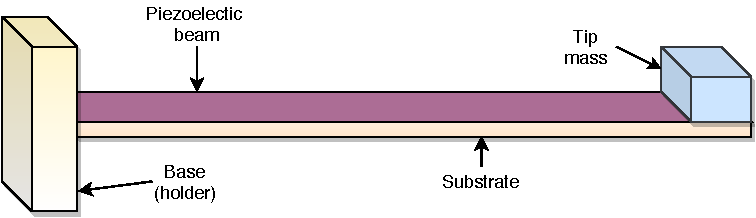
\includegraphics[scale=1]{beam1.pdf}
\end{figure}

\subsection{Efficiency and power density}
Piezoelectric generator is truly a non-linear device. It produces maximum output power at its resonance frequency, which depends on a number of factors. 
\par
Power density of the harvesters is expressed as the output power divided by the device volume for the given input \cite{EnHv2}. In case of vibrational energy, the input is the acceleration level and the frequency. An output of the piezoelectric generator provides voltage levels suitable for many electronics systems, therefore it is often unnecessary to add additional power electronics, what has an influence on efficiency.
\par
\begin{table}[ht!]
\small
\begin{center} 
\begin{tabular}{|c|c|c|c|l|}
\hline 
\textbf{Type} & \textbf{Conditions} & \textbf{Power Density} & \textbf{Area or Volume} & \textbf{Energy/Day} \\ 
\hline 
\hline
Vibration & $1m/s^2$ & $100\mu W/cm^3$ & $1cm^2$ & $8.64J$ (continuous vibration) \\ 
\hline 
Solar & Outdoors & $7500\mu W/cm^2$ & $1cm^2$ & $324J$ (sunny half a day) \\ 
\hline 
Solar & Indoors & $100\mu W/cm^2$ & $1cm^2$ & $4.32J$ (sunny half a day) \\ 
\hline 
Thermal & $\Delta T = 5 ^{\circ} C$ & $60\mu W/cm^2$ & $1cm^2$ & $2.59J$ (heat available for half a day) \\ 
\hline 
\end{tabular} 
\end{center}
\caption{Common data for some of Energy Harvesting Sources \cite{EnHv1}}
\label{tab:typdat}
\end{table}
\par

\subsection{Clamping}
Effective clamping is really important for piezoelectric beams. In order to achieve best performance, it is crucial to provide proper holder that gives reliable operation regardless of vibration level - see Figure \ref{fig:clamping}.\par

\begin{figure}[ht!]
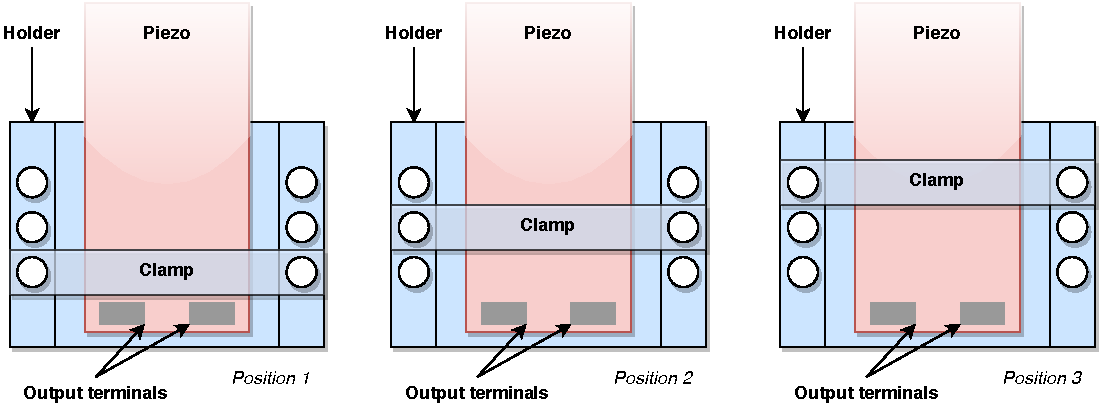
\includegraphics[scale=0.85]{clamping.pdf}
\caption{Clamping problem explanation}
\label{fig:clamping}
\end{figure}

For the sake of this project, the holder provided by the manufacturer would be used for evaluation purposes. The clamp bar is going to hold the beam in place with help of bolts and washers.\par
According to the manufacturer's datasheet \cite{PPA}, the second position of the clamp is a default configuration for all products. The third position of the clamp comes in handy when one need to increase the resonant frequency of the piezo wafer. On the other hand, the first position reduces the resonant frequency. It is noted that this hardware configuration is not recommended for energy harvesting applications due to stiffness issues.\par

\subsection{Tip mass}
Piezoelectric energy harvesters are frequency-dependent devices. In order to achieve their maximum efficiency, it is necessary to operate close to its resonant frequency. Piezoelectric beams may need some tuning procedures in order to match the frequency of the vibrating source, thus allowing to ensure most energy efficient harvesting.\par

\begin{figure}[ht!]
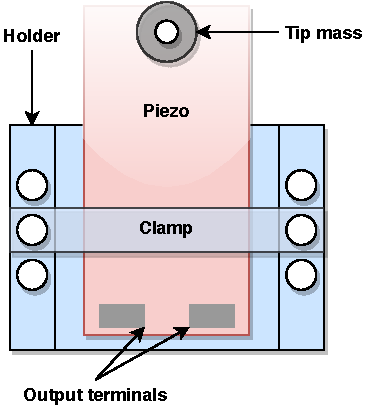
\includegraphics[scale=0.85]{tipmass.pdf}
\caption{Tip mass illustration}
\label{fig:tipmass}
\end{figure}

As mentioned in the previous subsection, frequency tuning may be performed by changing the clamp position. Unfortunately, this option does not allow for precise trimming, therefore additional techniques are often required. One of the most popular ones incorporated the tip mass attached at the end of the piezoelectric wafer. Providing that the operating frequency is fixed and known, it is possible to determine the exact tip mass required to tune the beam.
\par

In this case, $m$ is the effective mass, $m_k$ is the added tip mass, $k$ is the effective stiffness and $f$ is the natural frequency. One should take into account that these equations are valid only when the applied tip mass is centered and places according the the manufacturer's guidelines.

\begin{equation}
    f = \frac{\sqrt{\frac{k}{m + m_{t}}}}{2\cdot\pi}
    \label{resonant1}
\end{equation}

\begin{equation}
    m_{t} = \frac{k}{(2\cdot\pi\cdot f)^2} - m
    \label{resonant2}
\end{equation}

It is important to note that the natural frequency of the piezoelectric material is affected by such factors as temperature, manufacturing process, clamping conditions as well as vibration amplitude \cite{PPA}. Moreover, the resonance frequency is highly affected by the load powered by the harvester. 
\par

\subsection{Piezo beam resonance conditions}

To determine the natural frequency of the beam, one should apply a mechanical impulse to the beam and monitor its response. In order to do so, it is handy to use an oscilloscope in order to monitor the output of the loaded piezoelectric beam. The frequency of the decaying wave is equal to the natural frequency of the beam \cite{PPA}.
\par

\section{Measurement setup design}

A proper measurement process is a crucial part of this project. Having said that, a custom data acquisition board is to be designed. 
\par

First of all, it is vital to highlight most important features required to achieve desired performance. There are four major aspects that have to be taken into account, namely, the ADC resolution as well as the input voltage range, the bandwidth and high input impedance of the analog front-end. Apart from that, one should take care of easy interfacing to personal computer, thus compact size and USB interface would be considered as huge assets.
\par
The previous paragraph introduced briefly main functionalities of the target device. It is quite easy to notice that there would be a lot of trade-offs to consider through the design process. Compact size and the complex analog circuitry usually do not mix, especially when planning to get a device of USB mass storage size. These facts are forcing the designer to look for a microcontroller that provides decent ADCs, also in terms of the sampling rate. Since the project is dealing with piezoelectric generators, there is always a risk of relatively high voltages at the input terminals, especially when harvesters are not connected to any load. To face this problem, the data acquisition board would be equipped with two different means of protection. The first one takes care of the input stage of the device. The second one is a classic galvanic isolation between the microcontroller (as well as the analog front end) and the personal computer. This way, there is no risk of damaging host devices utilizing the data acquisition system. The summary of the above-mentioned description is presented in the Figure~\ref{fig:meas_overview}.\par

\begin{figure}[h!]
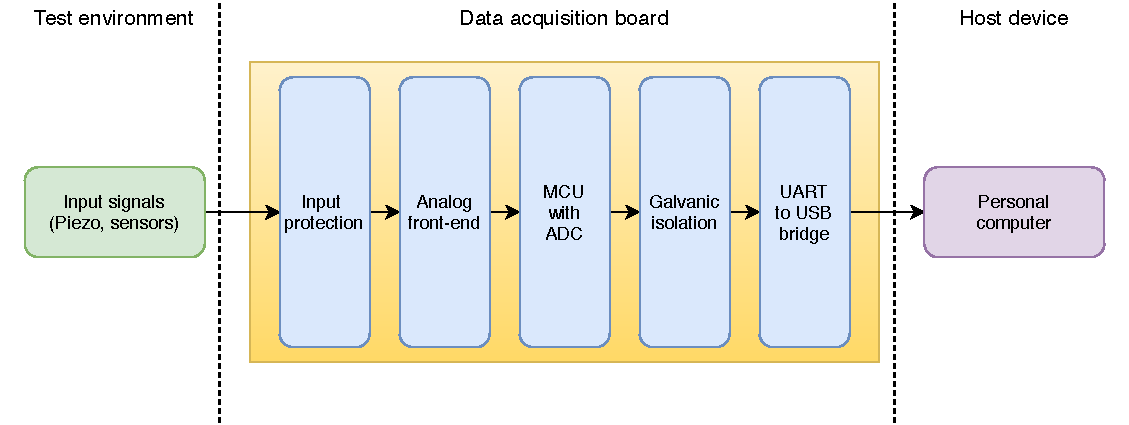
\includegraphics[scale=0.8]{measurement_setup_overview.pdf}
\caption{Measurement setup overview}
\label{fig:meas_overview}
\end{figure}

\subsection{Design requirements}
The first step of the design process is to determine desired input ratings as well as data acquisition capabilities. The piezoelectric device used in this project would be the major signal source during all experiments. Its datasheet \cite{PPA} does not state any fixed maximum ratings. Instead, it provides exemplary results obtained by varying acceleration amplitude, frequency, tip mass and load resistance - see Table \ref{tab:ppapower}.\par

\begin{table}[ht!]
\centering
\begin{tabular}{|c|c|c|c|c|c|c|}
\hline
\multicolumn{1}{|c|}{\textbf{\begin{tabular}[c]{@{}c@{}}Acceler.\\ ampl. $(g)$\end{tabular}}} & \multicolumn{1}{c|}{\textbf{\begin{tabular}[c]{@{}c@{}}Freq.\\ $(Hz)$\end{tabular}}} & \multicolumn{1}{c|}{\textbf{\begin{tabular}[c]{@{}c@{}}Tip mass\\ $(gram)$\end{tabular}}} & \multicolumn{1}{c|}{\textbf{\begin{tabular}[c]{@{}c@{}}RMS\\ power $(mW)$\end{tabular}}} & \multicolumn{1}{c|}{\textbf{\begin{tabular}[c]{@{}c@{}}RMS\\ voltage $(V)$\end{tabular}}} & \multicolumn{1}{c|}{\textbf{\begin{tabular}[c]{@{}c@{}}RMS\\ current $(mA)$\end{tabular}}} & \textbf{\begin{tabular}[c]{@{}c@{}}Load\\ $(k\Omega)$\end{tabular}} \\ \hline
0.25                                                                                                 & 132                                                                                    & 0.0                                                                                     & 0.1                                                                                    & 1.1                                                                                     & 0.1                                                                                      & 17.9                                                                 \\
0.50                                                                                                 & 131                                                                                    & 0.0                                                                                     & 0.2                                                                                    & 1.9                                                                                     & 0.1                                                                                      & 18.3                                                                 \\
1.00                                                                                                 & 131                                                                                    & 0.0                                                                                     & 0.7                                                                                    & 3.4                                                                                     & 0.2                                                                                      & 15.7                                                                 \\
2.00                                                                                                 & 129                                                                                    & 0.0                                                                                     & 2.2                                                                                    & 5.4                                                                                     & 0.4                                                                                      & 13.0                                                                 \\ \hline
0.25                                                                                                 & 60                                                                                     & 1.9                                                                                     & 0.1                                                                                    & 2.9                                                                                     & 0.0                                                                                      & 61.0                                                                 \\
0.50                                                                                                 & 60                                                                                     & 1.8                                                                                     & 0.5                                                                                    & 3.3                                                                                     & 0.2                                                                                      & 20.8                                                                 \\
1.00                                                                                                 & 60                                                                                     & 1.7                                                                                     & 1.8                                                                                    & 7.1                                                                                     & 0.3                                                                                      & 28.6                                                                 \\ \hline
0.25                                                                                                 & 22                                                                                     & 22.8                                                                                    & 1.4                                                                                    & 9.0                                                                                     & 0.1                                                                                      & 60.4                                                                 \\
0.50                                                                                                 & 22                                                                                     & 22.8                                                                                    & 4.4                                                                                    & 17.3                                                                                    & 0.3                                                                                      & 67.6                                                                 \\ \hline

\end{tabular}
\caption{Exemplary piezoelectric harvester response. Data from PPA-1001 datasheet \cite{PPA}}
\label{tab:ppapower}
\end{table}

As mentioned in the previous paragraph, there is no constrained area in terms of vibration frequency and level stated by the manufacturer. Based on the data presented in the Table \ref{tab:ppapower}, the designer is relatively free to determine the operating frequency range as well as input signal range recorded at at the harvester's output. When considering bandwidth and sampling rate, it is important to take into account the Nyquist criterion. It states that the sampling rate has to be twice the highest frequency in the signal \cite{ElEx}. Assuming maximum vibration frequency of 500Hz, more than 1000 samples per second need to be captured.
\par

Of course, this sampling rate only allows to reproduce an incoming signal (sinusoidal wave) as a corrupted triangle, since there is not enough data points to accurately reflect the sine shape. To solve this problem, the sampling rate should be increased by factor of 5 or so, what ultimately yields at least 5000 samples per second (sps). To illustrate the problem, Figure \ref{fig:nyquist} is introduced. It can be easily seen that sampling rate as high as twice the input signal frequency is definitely not enough. Having said that, the minimum expected sampling rate is to be at least 5000 sps.
\par

\begin{figure}[h!]
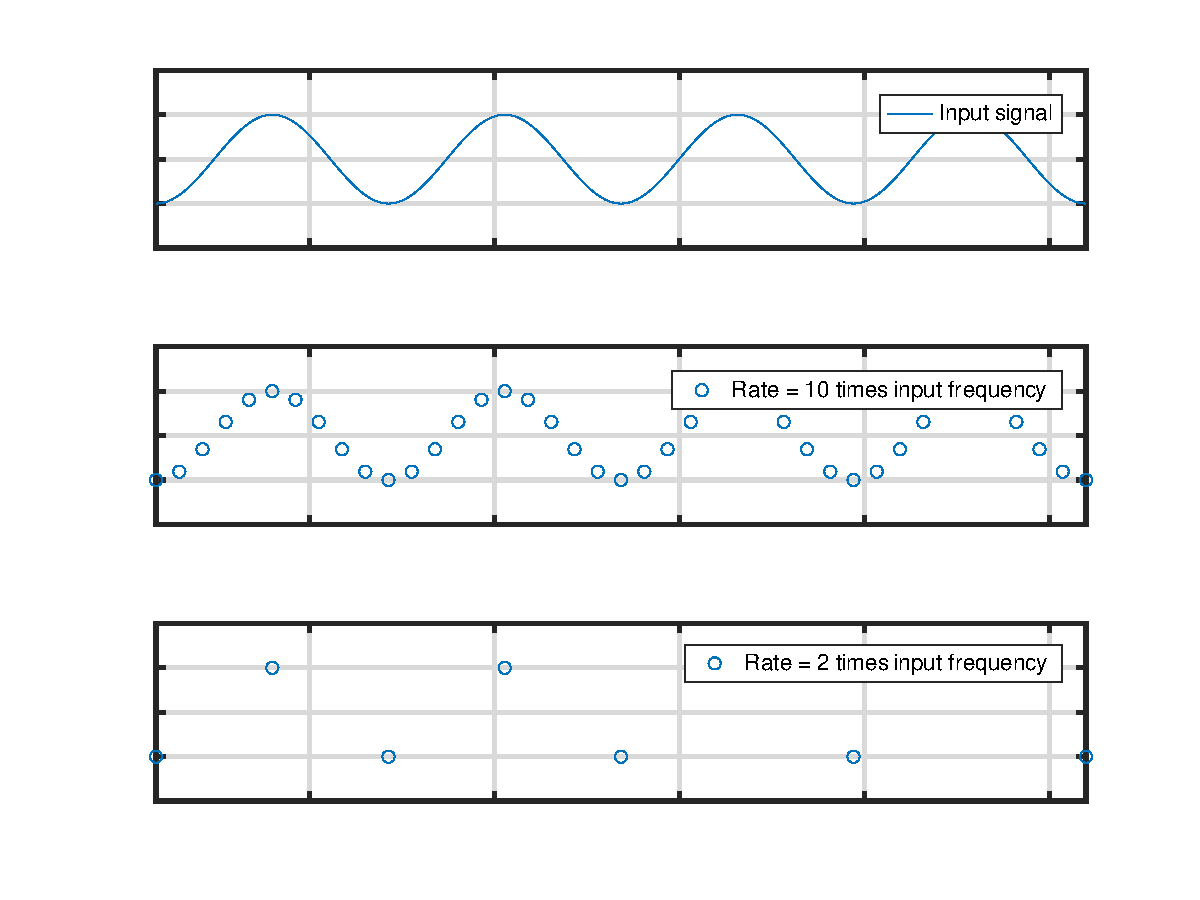
\includegraphics[scale=0.75]{nyquist.pdf}
\caption{Captured waveform versus sampling rate}
\label{fig:nyquist}
\end{figure}

It is likely that the microcontroller used in the data logger would use some kind of a serial communication protocol. Assuming that more than one signal is recorded at the time and the baud rate is fixed at the same level, the maximum input signal frequency would be divided by the number of active channels. For example, for 2 channel measurement, the maximum input signal frequency is 250Hz and so on.
\par

One of the previous paragraphs mentioned the piezoelectric harvester as the main input signal source. Knowing that the device produces a sinusoidal output, the analog front-end has to be able to capture AC signals, preferably of a relatively high amplitude. This requirements force the designer to develop symmetrical power supply for the input section as well as the circuitry allowing to add offset to the signal before it reaches the ADC input. A reason is that the ADC of the microcontroller is likely to accept only unipolar signals within tightly specified range. Remaining channels would be able to interface DC signals only, what makes them suitable for external sensors such as the accelerometer.
\par

When considering the maximum input signal level, one has to note that it should not exceed supply voltage of operational amplifier used in the input section. In case of the designed device, the power supply would be industrial $\pm{15}VDC$, as it helps to maintain compatibility with wide range of available operational amplifiers. Based on the last sentence, the maximum input voltage is specified to $\pm{15}V$ for the AC input and $+{15}V$ for DC inputs. In order to assure proper operating conditions for the analog-front end, an additional input protection is to be provided.
\par
There are two last aspect that need some care. The first one is the resolution of the ADC that would be used to capture the incoming signal. The second one is the input impedance of input channels.
\par
As to the first point, it is useful to have a look at technical details of commonly available oscilloscopes, since they can be treated as a nice reference. Most of them utilize 8 or 10-bit ADCs, mostly because of bandwidth requirements as well as the sampling time. In case of this design, the bandwidth is significantly reduced, what allows to look for a bit more resolution, of course still bearing in mind that all the processes are handled by one modest microcontroller. Putting it all together, an 14-bit ADC is going to be a desired data converter.
\par
The last point relates to the impedance of analog inputs. Piezoelectric harvesters are high output impedance devices \cite{EnHv1}, therefore it is desirable to maintain as high input impedance of the analog front-end as possible, in order not to disturb the incoming signal. There are two potential problems that may occur when designing the input stage. As it can be guessed, the input signal has to be divided before it gets to the analog-to-digital converter. The easiest way to go is to put a voltage divider directly at the output of the harvester. Unfortunately, this circuit would have a significant influence on the impedance seen from piezo generator's output terminals, thus posing a risk of changing its operating conditions. To deal with this problem, the incoming signal is to be buffered before any further processing. This is where low input bias current operational amplifiers would come in handy. The second risk is related to the protection circuitry attached to input terminals. Once the input signal gets to high, it would be clamped in order to protect the data acquisition board. Unhappily, it would also disturb the measured object due to rapid change of the impedance seen at mentioned harvester's output terminals. The only way to deal with this issue is to provide relatively high supply voltage for buffering amplifiers and adjust the load as to meet the input voltage requirements.
\par

As a summary of design considerations included in this subsection, Table \ref{tab:requirements} has been created.
\begin{table}[ht!]
\begin{tabular}{|l|c|}
\hline
\textbf{Requirement}              & \textbf{Value} \\ \hline
Max. input signal frequency (Sine) & 500Hz          \\ \hline
Min. sampling rate                 & 5000sps        \\ \hline
Min. ADC resolution                & 14-bit         \\ \hline
Max. input voltage range (p-p)     & 15V            \\ \hline
Input impeadnce                    & TBD            \\ \hline
\end{tabular}
\caption{Summary of requirements for the data acquisition board}
\label{tab:requirements}
\end{table}
\par

\subsection{Accelerometer board}
As it has been previously mentioned, is is necessary to constantly monitor vibration level during all the experiments. These measurements will be a reference for the results obtained using the piezoelectric harvester, as they easily allow to correlate generated power and current vibration level.
\par

The piezoelectric beam used throughout the research is mounted in a 3D-printed holder provided by the device manufacturer. Apart from a proper fit, it allows to attach some external electronics by means using nice mounting holes. It is worth to take advantage of this feature, therefore designed electronics would be compatible with the handler.
\par

\subsubsection{Most important parameters of the accelerometer}
As to the electrical and electromechanical properties of the accelerometer, there are a few aspects that should be highlighted. The first one is the measurement range. By checking the maximum acceleration of the beam, it is possible to estimate required range for the sought integrated circuit. Next, the frequency response and output signal type need to be determined. Frequency response describes the measurement resolution that could be understand as the smallest detectable acceleration \cite{accel_params}. By mentioning the type of the output signal, it was intended to distinguish between analog and digital output types. It is planned to synchronize the accelerometer output with the piezoelectric cantilever response, so the analog output is more suitable and easier to use.
\par
Harvester's datasheet \cite{PPA} does not mention the exact upper limit of allowed vibration level. According to the Table \ref{tab:ppapower}, the maximum acceleration amplitude mentioned by the manufacturer is 2g. Without any additional information, it is reasonable to treat this value as the upper acceleration limit. The same applies to the frequency response, which is also not described precisely. Again, Table \ref{tab:ppapower} states the maximum operation frequency at the level of 132Hz. In this case, the minimum acceptable bandwidth of the accelerometer would be roughly 200Hz. As it was mentioned in the previous paragraph, it is intended to use the analog output accelerometer. A summary of the above-mentioned choices is presented in the Table \ref{tab:accel_requirements}.

\begin{table}[ht!]
\begin{tabular}{|l|c|}
\hline
\textbf{Requirement}            & \textbf{Value} \\ \hline
Max. acceleration value  		& $\pm{2}g$         \\ \hline
Max. operating frequency        & 300Hz        \\ \hline
Output type             		& Analog         \\ \hline
\end{tabular}
\caption{Summary of requirements for the accelerometer}
\label{tab:accel_requirements}
\end{table}
\par

\subsubsection{Selection of the integrated circuit}
After a thorough market research, a proper device has been found - see Table \ref{tab:adxl_params}. Apart from parameters listed in the table, the selected accelerometer has the following features: small SMD package, 3.3V supply operation, low power consumption and tunable bandwidth filters for every axis. Moreover, it exhibits non-linearity at a level of 0.3$\%$ \cite{ADXL}.
\par

\begin{table}[ht!]
\begin{tabular}{|l|c|}
\hline
\textbf{Parameter}		& \textbf{Value} 	\\ \hline
Model  					& ADXL335         	\\ \hline
Manufacturer        	& Analog devices	\\ \hline
Output type           	& Analog  			\\ \hline
Max. acceleration value &  $\pm{3}g$		\\ \hline
Bandwidth 				&  up to 1600Hz		\\ \hline
\end{tabular}
\caption{Parameters of the selected parameter - taken from the datasheet \cite{ADXL}}
\label{tab:adxl_params}
\end{table}

As it can be seen, the above-mentioned device fulfils the requirements presented in the previous subsection. At this point, it is necessary to think about additional circuitry allowing to take advantage of the selected integrated circuit. In order to do so, a small PCB is to be designed.
\par

\subsubsection{Accelerometer board design}
The accelerometer board should be a battery powered device, as it is going to be used throughout tests in different types of environment, many times without an access to any power supply. Moreover, battery operation allows for a better performance in terms of noise generated on supply rails. Additionally, the board is ought to be equipped with a temperature sensor, in case some tests are to be performed in extreme temperatures and the exact temperature value is needed to know.
\par
Figure \ref{fig:accel_diagram} presents the diagram of designed board. It can be divided into two main parts, namely a power supply with a battery charger and a sensing part including the accelerometer and the temperature sensor.
\par


\begin{figure}[ht!]
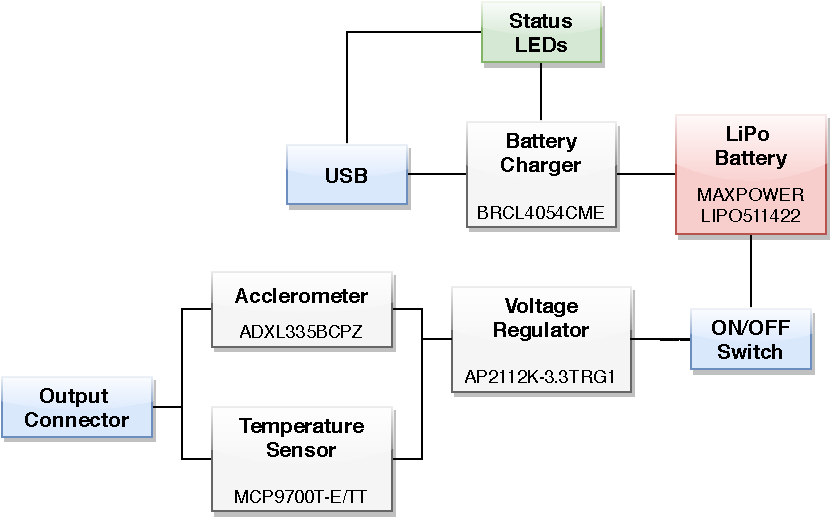
\includegraphics[scale=1]{accel.pdf}
\caption{Accelerometer board diagram}
\label{fig:accel_diagram}
\end{figure}

\begin{figure}[ht!]
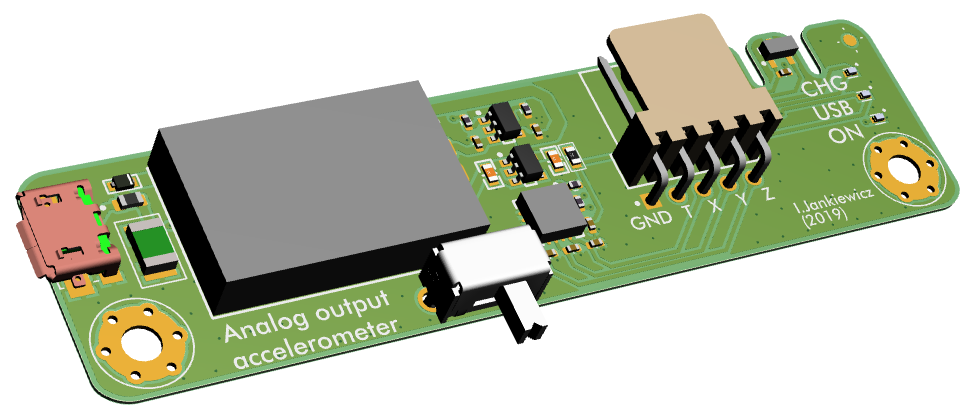
\includegraphics[scale=0.6]{accelerometer1.png}
\caption{Accelerometer board top side view}
\label{fig:accel1}
\end{figure}

\begin{figure}[ht!]
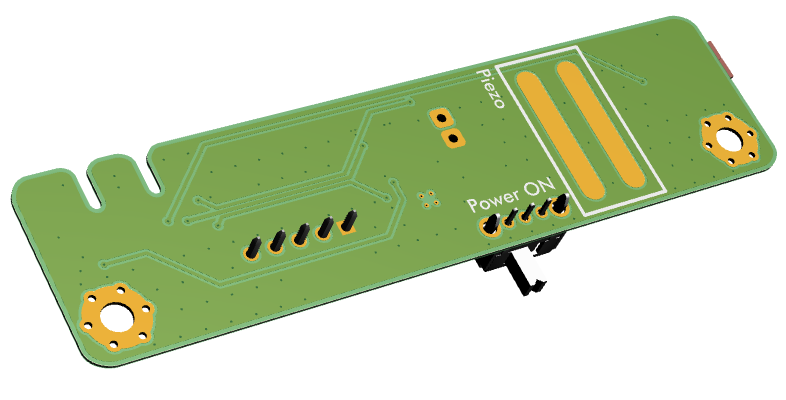
\includegraphics[scale=0.7]{accelerometer2.png}
\caption{Accelerometer board bottom side view}
\label{fig:accel2}
\end{figure}
\par 

As to the power supply part, for the convenience, the entire board in powered using a micro USB port, which is fused for safety purposes. Right after the input, there is a single cell battery charger (BRCL4054CME by Blue Rocket Electronics \cite{charger_params}). Charging current is set using just one resistor. Moreover, it incorporates such function as C/10 charge termination, a soft-start feature as well as an open-drain output used for signalling purposes.
\par
Power storage is maintained by means of a 110mAh lithium-polymer battery (LIPO511422 by MAXPOWER). It is equipped with a complete protection circuitry, so it is unnecessary to include additional protection on the accelerometer board. The battery manufacturer claims the cycle life of 1000 cycles.
\par

Right after the ON/OFF switch, there is a low dropout linear regulator supplying the rest of circuits (AP2112K-3.3TRG1 by Diodes Incorporated \cite{ap2112_params}). It is a 600mA output, low noise regulator with $\pm{1}\%$ output voltage accuracy.
\par

One of the sensors placed on this board is the accelerometer mentioned in the previous section. The second one is a low-power linear temperature sensor (MCP9700T-E/TT by Microchip \cite{mcp9700_params}). Since the linear output is one of the requirements for all sensors used in this project, this kind of device was an easy choice. MCP9700 includes circuitry converting temperature to voltage and provides accuracy of $\pm{2}^\circ $C, which is by all means acceptable for this application.
\par

Figures \ref{fig:accel1} and \ref{fig:accel2} present the final design. As it can be seen, a relatively compact and intuitive device has been developed. A standard connector with 2.54mm pitch is used to allow easy access to the board. There are two reinforced holes for mounting screws. The bottom side of the PCB includes large past allowing to solder cables connected to piezoelectric beam terminals in order to make the construction more robust.
\par

This board is going to be an inherent part of most experiments performed throughout this thesis.
\par

\subsection{Data acquisition board design}
\subsubsection{AC input section}
The data acquisition board is going to be equipped with one AC-tolerant input channel. This feature will be helpful in cases when piezoelectric beam is loaded only with a resistive load, hence there is no rectification action present. In order not to damage the microprocessor and other circuitry that is powered from a single supply, some signal conditioning is required. 
\par
\paragraph{Input protection}
An important aspect (often overlooked though) is proper input protection for analog circuitry. At this point it is important to highlight that signal conditioning would be based on a variety of different operational amplifiers. Having said that, one should consider problems related to these devices as well as the influence of protection circuit on measurement results.
\par

One of most popular means of protection for op-amps are clamping diodes along with current limiting resistors. Nowadays, popular operational amplifiers incorporate ESD protection diodes into their input circuitry, which is surely very helpful in most cases, nevertheless it can be a source of potential problems. These diodes are clamped to supply rails in order to provide return path for currents generated by ESD-related events. These happen once the input voltage gets higher than supply rail voltage plus voltage drop (usually around 0.7V) or lower than negative rail voltage minus the diode voltage drop, respectively \cite{clamping}. In normal conditions these diodes remain transparent. 
\par

It is important to remember that the clamping circuit is going to have an influence on measurement results if designed improperly. Now, it is time to recall a very important parameter related to inputs of the operational amplifier, namely the Input Bias Current $I_{bias}$, which is inherently related to any "real" (and non-ideal) Op Amp. It's value is going to have a direct influence on the clamping circuit design, what would be explained in a more detailed manner soon.
\par

\begin{figure}[ht!]
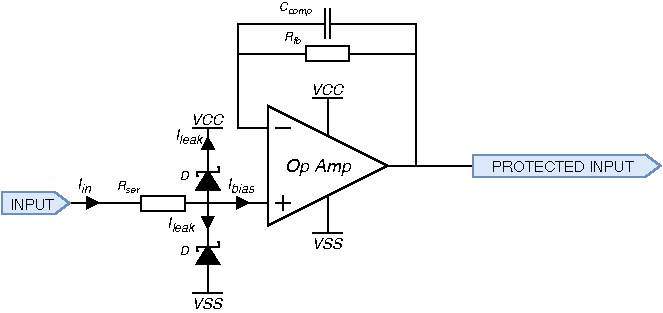
\includegraphics[scale=1.2]{input1.pdf}
\caption{Clamping overvoltage protection scheme}
\label{fig:input1}
\end{figure}

The Input Bias Current $I_{bias}$ is a DC current required by the Op Amp's inputs to establish proper biasing of input stage transistors \cite{companion}. It ranges from a few picoamps to a few microamps. This current is going to flow through the series protection resistor, generating a voltage drop proportional to mentioned current value multiplied by the series resistance. The explanation is presented in the Figure \ref{fig:input1}.
\par

Another unwanted, but also unavoidable error source is the Reverse Leakage Current $I_{leak}$ of clamping diodes, which depends on the value of reverse voltage applied to its terminals.
All unwanted currents add up and flow through the series protection resistor $R_{ser}$ generating the voltage drop. The total error voltage $V_{error}$ is equal to the mentioned voltage drop multiplied by the gain of the operational amplifier $A_u$ - see Equation \ref{bias}.

\begin{equation}
    V_{error} = (R_{ser} \cdot (I_{bias} + I_{leak1} +  I_{leak2})) \cdot A_u
    \label{bias}
\end{equation}
\par

Of course, apart from the error generation, the clamping circuit plays a crucial role in operational amplifier's inputs protection, since it allow to deal with excessive voltage without any problems. The maximum continuous input voltage can be calculated if the value of series resistance, the Forward Continuous Current $I_f$, op-amp supply voltage $V_{cc}$ and the diode forward voltage drop $V_{fd}$ are known. Peak input voltages can even be even higher, as this parameter depends strongly on the current value flowing through the protection diode.
\begin{equation}
    V_{in(MAX)} = V_{cc} + R_{ser} \cdot I_f + V_{fd}
    \label{maxvolt}
\end{equation}
\par 
To summarize, it is vital to emphasize once again the importance of the champing circuit. Even though it can introduce some error, careful component selection allows to find the balance between the performance and protection properties. It is important to use Schottky diodes, as only low voltage drop devices ale able to bypass the internal ESD protection diodes placed at inputs of the op-amp, what ultimately prevents from unintended damage of the protected device.
\par
Taking into account all information included in this paragraph, a proper clamping diode has been chosen. Its parameters are presented in the Table \ref{tab:bas40_params}.

\begin{table}[ht!]
\begin{tabular}{|l|c|}
\hline
\textbf{Parameter}		& \textbf{Value} 	\\ \hline
Model  			& BAS40-02V-V-G         	\\ \hline
Manufacturer    & Vishay Semiconductors	\\ \hline
Type           	& Schottky  			\\ \hline
Package &  SOD-523		\\ \hline
Repetitive peak reverse voltage $V_{RRM}$ &  40V \\ \hline
Forward continuous current $I_{F}$ &  120mA \\ \hline
Leakage current $I_{R}$ &  20nA (Typ.) \\ \hline
Forward voltage $V_{F}$ &  380mV ($I_F$=1mA) \\ \hline
\end{tabular}
\caption{Parameters of the selected parameter - taken from the datasheet \cite{bas40_params}}
\label{tab:bas40_params}
\end{table}

\paragraph{Buffering}

This project is all about high impedance signals, what automatically forces designer to make the analog front-end "invisible" for the signal source. In order to do so, the input stage of the data acquisition board is supposed to draw as little current as possible. 
\par

The design requirements states the maximum peak-to-peak input voltage as high as 12V. This fact obliges to supply operational amplifiers using at least industry's standard $\pm$15V rails, providing that op-amps used in the project would not get saturated. Rail-to-rail devices may be helpful in this situation.
\par
Figure \ref{fig:input1} presents the exact configuration of the op-amp circuit. It is called a voltage follower or a buffer. At this point, it is very important to once again look at the estimated current consumption of the input stage. Previous paragraph stated all unwanted current paths that deteriorate the performance of the entire circuit. The leakage current $I_{leak}$ of diodes should be kept as low as possible (in order of nanoamperes). The another error source highlighted before is the input bias current $I_{bias}$ of the operational amplifier's non-inverting input. Since the buffer circuit is used, the input impedance of the amplifier is limited by the $I_{bias}$ only. Modern op-amps can draw as little bias current as a few picoamperes, therefore, the impact of this device is negligible providing that the proper integrated circuit will be used.
\par

When designing op-amp circuits, it is important to match the impedance of both inputs in order to avoid output voltage offsets. In case when these impedances are not equal, offset voltages generated by the bias current of both inputs have no chance to cancel out, introducing another error source \cite{companion}. The compensating capacitor $C_{comp}$ used in the feedback network (along with the feedback resistor $R_{fb}$) is forming an RC filter slowing down the amplifier's response and making it more stable, but it is necessary to keep its resonant frequency at reasonable level in order not to disturb the input signal.
\par

After a market research, the appropriate operational amplifier has been found - see Table \ref{tab:OPA4180_params}. At this point is possible to calculate the error voltage introduced by the input protection circuitry using Formula \ref{bias}. Please note that it is the worst case scenario, when both diodes exhibit maximum leakage current.
\begin{align}
\nonumber  V_{error} & = (R_{ser} \cdot (I_{bias} + I_{leak1} +  I_{leak2})) \cdot A_u
\\ \nonumber & = (1k\Omega \cdot (250pA + 20nA + 20nA))\cdot 1
\\ \nonumber & = 40.25\mu V
\end{align}
Of course, it is just a simple calculation that excludes such factors as temperature impact, tolerance of the resistor and so on. Having said that, the above-mentioned value is presented just to indicate the order of expected error.
\begin{table}[ht!]
\begin{tabular}{|l|c|}
\hline
\textbf{Parameter}		& \textbf{Value} 	\\ \hline
Model  			& OPA4180         	\\ \hline
Manufacturer    & Texas Instruments	\\ \hline
Supply voltage           	& $\pm$2V to $\pm$ 18V  			\\ \hline
Bias current &  250pA (typical)		\\ \hline
Input offset voltage &  75$\mu$V (maximum) \\ \hline
Drift voltage &  0.1$\mu$V/ \degree C \\ \hline
Input voltage noise &  0.25$\mu V_{pp}$ \\ \hline
Slew rate &  0.8V/$\mu$s \\ \hline
\end{tabular}
\caption{Parameters of OPA4180 taken from the manufacturer's datasheet \cite{bas40_params}}
\label{tab:OPA4180_params}
\end{table}
\par
\paragraph{Signal conditioning}
A first step in capturing the incoming signal was buffering. Now, the signal has to be conditioned in order to allow full range measurement. As it can be imagined, the input range of popular mictrocontroller's ADCs is usually up to 5V and more often up to 3.3V. This fact introduces a need of some attenuation and biasing, since an AC signal is considered.
\par 

Attenuation is going to be performed by means of a voltage divider. Unfortunately, there are a few problems that may appear in this solution. The first one is the excessive loading of the circuit. High current is going to generate losses in a form of heat. Any resistor has a parameter called temperature coefficient, which describes the resistance change in a function of temperature (usually in ppm/$^\circ$C) \cite{housekeeping}. High temperature coefficient components are undesired in precision electronics, thus designers should avoid them by all means.   Temperature-related problems could be solved in a couple of different ways. In case of this design, the voltage divider would consist of low temperature coefficient resistors buffered with an operational amplifier. This solution would allow for a negligible current draw. The Op Amp used for this purpose is exactly the same as in case of the input buffer - see Table \ref{tab:OPA4180_params}.
\par

At this point, it is time to introduce the signal biasing. This process is absolutely necessary, since the microcontroller is unable to capture negative voltage. This stage takes into account such aspects as input voltage range of the ADCs as well as the reference voltage value, as its value determines the maximum signal level distinguishable by the microprocessor.

\begin{figure}[ht!]
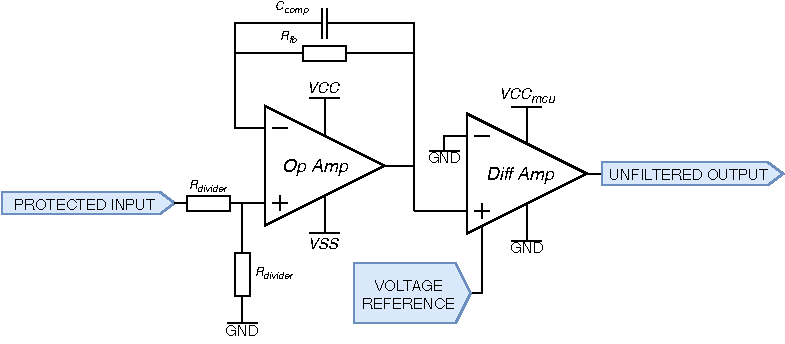
\includegraphics[scale=1.2]{input2.pdf}
\caption{A circuit responsible for attenuation and level shifting}
\label{fig:input2}
\end{figure}

\subsubsection{Voltage reference}

The reference voltage source is an important building block in precision analog electronics. Due to the fact that the designed board utilizes the analog-to-digital converter with resolution of at least 14-bits, it is important to follow particular design rules in order not to spoil its performance.
\par

There are many different flavours of voltage reference sources, but the basic division includes zener and band-gap reference types \cite{companion}. Zener-based voltage incorporates a low-tempco zener diode and additional circuitry such as a matching silicon diode cancelling the influence of the temperature coefficient. Quite often, such references include internal heaters in order to maintain relatively stable temperature of the diode, therefore reducing the temperature impact. It is worth to highlight that such references may get quite expensive and very often offer only high reference voltage values, thus some additional circuitry may be required for interfacing the a microcontroller \cite{companion}.
\par

The second type of voltage reference sources is called the band-gap reference voltage. This type is based on matched transistors, and with some additional circuitry, it is able to provide lower (and precisely trimmed) reference voltages with comparable temperature coefficients. Moreover, such references may include internal buffer, thus no additional circuitry is often required \cite{companion}.
\par

The most important parameters of the voltage reference source are the mentioned temperature coefficient and output voltage tolerances. Due to the fact that band-gap references   are readily available and offer suitable reference voltage levels, this type of solution would be considered in this design.\par

\begin{table}[ht!]
\begin{tabular}{|l|c|}
\hline
\textbf{Parameter}	& \textbf{Value} 	\\ \hline
Model  				& REF5030       \\ \hline
Manufacturer    	& Texas Instruments	\\ \hline
Temperature drift (max)       	&  8ppm/\degree C 	\\\hline
Output voltage tolerance (max)     &  0.1\%			\\ \hline
Output current (max)       & 10mA\\ \hline
Type         &  Band-gap				\\ \hline
Reference voltage value		&  3.0V		\\ \hline

\end{tabular}
\caption{Parameter of REF5030 taken from the manufacturer's datasheet \cite{ref5030_params}}
\label{tab:fer5030_params}
\end{table}

\subsubsection{Microprocessor selection}
The microcontroller is a brain of the data acquisition board. As it can be imagined, it is responsible for such tasks as analog-to-digital conversion, data processing and communication with a personal computer. In addition, it is going to provide a basic user interface by means of buttons and switches for configuration purposes and signalling LEDs. Apart from that, there should be some space for calibration process, as well as triggering signals, thus additional I/Os would be included on the board for user-friendliness.
\par

The Table \ref{tab:requirements} listed some of design requirements applicable for the MCU, namely, the ADC resolution as well as minimum sampling rate. In addition to that, the microprocessor has to be equipped with sufficient amount of inputs and outputs as well as communication interfaces in order to provide reliable connectivity with the PC.

\begin{table}[ht!]
\begin{tabular}{|l|c|}
\hline
\textbf{Parameter}	& \textbf{Value} 	\\ \hline
Model  				& MSP432P401R       \\ \hline
Manufacturer    	& Texas Instruments	\\ \hline
Architecture       	&  32-bit ARM 		\\ \hline
Clock frequency     &  48MHz			\\ \hline
Flash memory        &  256KB			\\ \hline
SRAM memory         &  64KB				\\ \hline
ADC resolution 		&  up to 16-bit		\\ \hline
ADC sampling rate 	&  up to 1Msps 		\\ \hline
ADC input channels 	&  up to 24  		\\ \hline
UART channels 		&  4 				\\ \hline
UART max. baud rate &  460800bps 		\\ \hline
SPI channels 		&  4 				\\ \hline
SPI max. baud rate &  16Mbps 			\\ \hline
\end{tabular}
\caption{Features of MSP432P401R taken from the manufacturer's datasheet \cite{msp432_params}}
\label{tab:MSP432_params}
\end{table}

\par
By following mentioned requirements, the device presented in the Table \ref{tab:MSP432_params} has been selected for this design. It is worth to highlight its superior analog features, namely the analog-to-digital converter capable of producing 16-bit results when the appropriate layout and averaging of recorded samples are implemented (the device incorporates a native 14-bit SAR core) \cite{16bit}. Apart from analog-related features, the selected MSP432 provides numerous digital interfaces, what comes in handy when a connection with a personal computer is required. In this design, the primary communication channel would be based on UART, but is also planned to include an SPI-to-USB bridge for experimental purposes.
\par

\paragraph{Architecture}
Once the right microcontroller has been selected, one has to think about its peripherals required to allow easy connectivity as well as user-friendly interface. A general architecture of the designed system is presented in the Figure \ref{fig:architecture}. In the following sections, all major sections would be briefly introduced.

\begin{figure}[ht!]
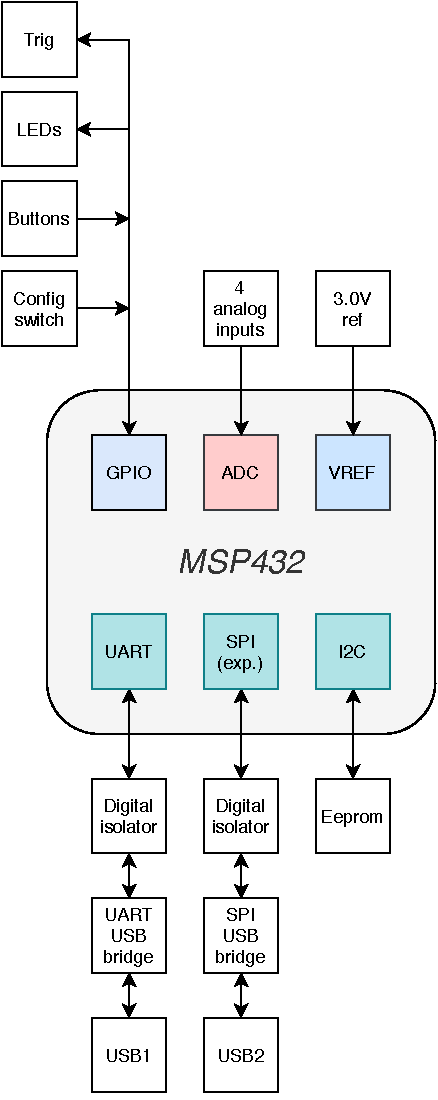
\includegraphics[scale=1]{architecture.pdf}
\caption{Architecture of the microcontroller and its peripherals}
\label{fig:architecture}
\end{figure}

\par

\paragraph{ADC}
The analog-to-digital converter is the most important part of the entire system. According to the manufacturer's description \cite{msp432_params}, the selected device is able to achieve 16-bit precision with software over-sampling. The sampling rate is resolution dependent and for 14-bit mode, MSP432 is able to provide 1Msps. It is vital to point out that for better precision, the external voltage reference source is used. 
\par

\paragraph{External voltage reference}
As mentioned in the previous paragraph, the MCU is equipped with the external reference voltage source in order to improve stability of the ADC. The selected device (REF5030)  provides such features as the accuracy as low as 0.1\% and temperature drift lower than 8ppm/\degree C \cite{ref5030_params}. The built-in reference has only 1\% accuracy and temperature drift up to 60ppm/\degree C \cite{msp432_params}. MSP432 devices provide dedicated voltage reference input terminals (+VREF and -VREF) to facilitate the described modification.
\par

\paragraph{User interface} 
The purpose of the data acquisition board is to allow easy and precise measurement of high impedance signals with a focus on piezoelectric-based circuits. The standard way of communication between the board and user is maintained by means of a personal computer, but there is some space for improvement.
\par
It is planned to incorporate some basic functionalities based on switches and buttons. A 4-channel DIP switch is designated for configuration purposes. There are also two momentary buttons allowing to control the measurement process. An RGB LED is used for status indication.
\par
In addition, there is a dedicated trigger pin that could be used to synchronize the board with a signal or with an external measurement instrument.
\par

\paragraph{Connectivity}
The designed device utilizes a few digital interfaces to communicate with peripherals and the personal computer. UART and SPI are used for data streaming and for parsing commands. I2C interface is used for communication with an EEPROM memory storing calibration constants and some basic info related to the device. At this point it is important to point out that SPI interface is for experimental purposes only, therefore UART is assumed to be the basic interface between the computer and the board.
\par
Since the data acquisition module is glvanically isolated from the computer, all signals has to include additional isolating devices. In case of the UART, Rx and Tx signals are separated between primary and secondary side of the board by means of an Analog Devices ADuM1201 digital isolator. According to the manufacturer's datasheet \cite{adum1201_params}, it supports data rates up to 25Mbps and 2500V RMS isolation for 1 minute per UL 1577. SPI interface is isolated using Maxim Integrated MAX14851 six-channel digital isolator. It is supporting data rates as high as 50Mbps and isolation of 600V RMS for 1 minute \cite{max14851_params}.
\par
In order to make the device compatible with USB protocol, it is necessary to provide signal bridges for UART and SPI interfaces. This way, the user would be able to easily connect the data acquisition board directly to the personal computer. The USB-to-UART bridge parameters are stated in the Table \ref{tab:cp2102_params}. It supports baud rates up to 1Mbps, which makes it suitable fot this design. It is important to point out that CP2012 is fully compatible with most popular operating systems.

\begin{table}[ht!]
\begin{tabular}{|l|c|}
\hline
\textbf{Parameter}	& \textbf{Value} 	\\ \hline
Model  				& CP2102       \\ \hline
Manufacturer    	& Silicon Labs	\\ \hline
Max. baud rate       	&  1Mbps 		\\ \hline
On-chip voltage regulator     &  3.3V			\\ \hline
USB 2.0 compliant        &  Yes			\\ \hline
Transmit buffer        &  640 bytes				\\ \hline
Receive buffer 		&  576 bytes		\\ \hline
USB powered 	&  Yes 		\\ \hline
Compatibility 	&  Windows/Linux/Mac  		\\ \hline
\end{tabular}
\caption{Features of CP2102 taken from the manufacturer's datasheet \cite{cp2102_params}}
\label{tab:cp2102_params}
\end{table}

The USB-to-SPI bridge is also manufactured by \textit{Silicon Labs} - see Table \ref{tab:cp2130_params}. The  most important features of this device are the maximum baud rate of 12MHz and 11 fully configurable GPIOs. Due to the fac2t that SPI is jut an experimental mean of communication is this project, there would be no more focus on SPI-related circuitry.

\begin{table}[ht!]
\begin{tabular}{|l|c|}
\hline
\textbf{Parameter}	& \textbf{Value} 	\\ \hline
Model  				& CP2130       \\ \hline
Manufacturer    	& Silicon Labs	\\ \hline
Max. SPI clock       	&  12MHz 		\\ \hline
On-chip voltage regulator     &  3.45V			\\ \hline
USB 2.0 compliant        &  Yes			\\ \hline
Operation modes        &  3 or 4-wire			\\ \hline
Configurable GPIOs 		&  11		\\ \hline
USB powered 	&  Yes 		\\ \hline
Compatibility 	&  Windows 		\\ \hline
\end{tabular}
\caption{Parameters of CP2130 taken from the manufacturer's datasheet \cite{cp2130_params}}
\label{tab:cp2130_params}
\end{table}

\begin{figure}[ht!]
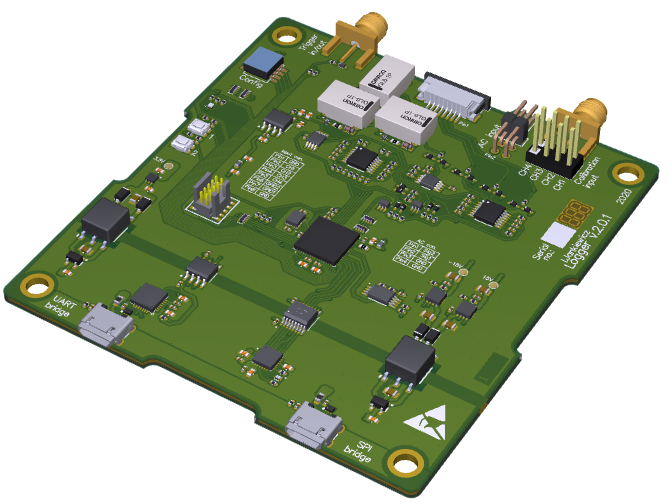
\includegraphics[scale=0.9]{logger.png}
\caption{Data acquisition board 3D model}
\label{fig:logger3d}
\end{figure}

\section{Energy harvester}
The second aspect of this Master's project is to investigate the concept of vibrational energy harvesting. In order to do so, a proper power conditioning circuitry is to be provided.

\subsection{Energy harvesting integrated circuits}
\subsubsection{LTC3588-1}
The \textit{LTC3588-1} by \textit{Linear Technology} is one of the most popular off-the-shelf solutions used in piezoelectic energy harvesting applications. Owing to the fact that target applications of such energy scavenging systems are focused on IoT devices, the described integrated circuit has one huge advantage in comparison to other devices, namely the solution size.
\par
It's datasheet \cite{ltc3588_params} states that to make the device work properly, only four capacitors and one inductor are required. Additional two resistors may be useful in order to set desired output voltage, but they are just an option. The simplified diagram of the described solution is presented in the Figure \ref{fig:ltc3588diagram}. It is worth to note that the solution size is greatly reduced by an integrated low-loss full-wave bridge rectifier that also makes a perfect fit for AC input signals.

\begin{figure}[ht!]
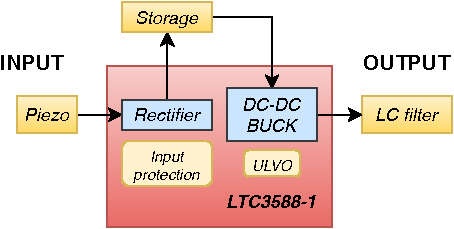
\includegraphics[scale=1.2]{LTC3588.pdf}
\caption{The diagram of \textit{LTC3588-1} based energy harvesting system}
\label{fig:ltc3588diagram}
\end{figure}

\par

Most important parameters of \textit{LTC3588-1} are mentioned in the Table \ref{tab:ltc3588_params}. Apart from the mentioned integrated rectifier, there are a few more features making this integrated circuit suitable for the job.  The input voltage range easily covers values expected at the output of simple piezoelectric generators. Moreover, it included an overvoltage clamp protecting the device \cite{ltc3588_params}. Very low quiescent current of the device makes it possible to use just a supercapacitor as an energy storage element.

\begin{table}[ht!]
\begin{tabular}{|l|c|}
\hline
\textbf{Parameter}	& \textbf{Value} 	\\ \hline
Model  				& LTC3588-1       \\ \hline
Manufacturer    	& Linear Technology	\\ \hline
Input operating range      &  2.7V to 20V 		\\ \hline
Quiescent current     &  950nA			\\ \hline
Output current        &  up to 100mA			\\ \hline
Selectable output voltages & 1.8V, 2.5V, 3.3V, 3.6V\\ \hline
Input protection &  Shunt type (up to 25mA Pull-down)\\ \hline
Undervoltage lockout 	&  Yes 		\\ \hline
Integrated rectifier 	&  Yes 		\\ \hline
\end{tabular}
\caption{Most important features taken from the manufacturer's datasheet \cite{ltc3588_params}}
\label{tab:ltc3588_params}
\end{table}
\par

\paragraph{Circuit design}
When designing low power circuits, great care has to be taken about proper storage components, as these are the key to maintain an uninterrupted output of these circuits. The input capacitor is responsible for providing sufficient amount of energy for the DC-DC converter. On the other hand, the output capacitor determines the time interval for which the converter sleeps \cite{ltc3588_params}. The exact size of mentioned components is mostly dependent on a particular application. Therefore, manufacturer's recommendation would be a reference in case of this design. Please note that selected components are supposed to meet voltage rating requirements, namely at least 20V for the input capacitor and 6.3V for the output capacitor. Based on these details, the following components have been picked:

\begin{table}[ht!]
\begin{tabular}{|c|c|c|c|c|c|}
\hline
 \textbf{Type} & \textbf{Manufacturer} & \textbf{Model} & \textbf{Capacitance} & \textbf{Rated voltage} & \textbf{Count}	\\ \hline
Input & Würth Elektronik & 865060442002 & 22$\mu$F & 25V & 1      \\ \hline
Output & AVX & 12066C226MAT2A  & 22$\mu$F & 6.3V & 3      \\ \hline

\end{tabular}
\caption{Capacitors selected for the \textit{LC3588-1} circuit \cite{x5r_params}, \cite{ltc3588_capacitor_params}}
\label{tab:ltc3588_capacitors}
\end{table}

When it comes to the inductance, the manufacturer advises to pick any value between 10$\mu$H and 22$\mu$H. Larger inductors can be beneficial in high voltage applications \cite{ltc3588_params}. The selected component should have a DC current rating of 350mA or more. Please note that DC resistance of the inductor has an impact on the overall efficiency of the converter.

\begin{table}[ht!]
\begin{tabular}{|c|c|c|c|c|}
\hline
\textbf{Manufacturer} & \textbf{Model} & \textbf{Inductance} & \textbf{Rated current} & \textbf{DC resistance}	\\ \hline
 Würth Elektronik & 74438335220 & 22$\mu$H & 0.6A & 1.04$\Omega$      \\ \hline

\end{tabular}
\caption{Inductor selected for the \textit{LC3588-1} circuit \cite{ltc3588_inductor_params}}
\label{tab:ltc3588_inductor}
\end{table}

\par

Figure \ref{fig:ltc3588layout} presents the layout of the described circuit. Apart from previously mentioned components, there is also a DIP switch allowing to configure the output voltage of the converter. This way, the DC-DC converter could be easily adjusted by the user according to the table printed on the silkscreen.

\begin{figure}[ht!]
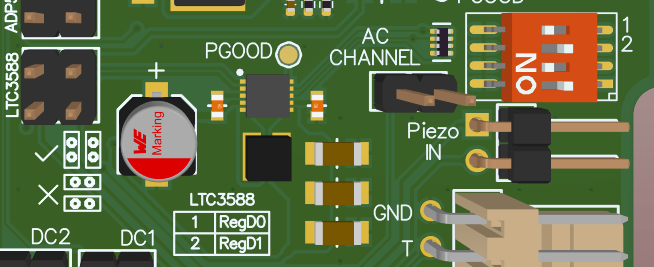
\includegraphics[scale=0.8]{ltc3588_layout.png}
\caption{The layout of \textit{LTC3588-1} based circuit}
\label{fig:ltc3588layout}
\end{figure}

\subsubsection{LTC3331}
The most complicated of integrated circuits selected for this design is \textit{LTC3331} by \textit{Linear Technology}. It takes advantage of a few features very similar features to those described in the section focused on \textit{LTC3588-1}, but its performance is extended. This notion would be described further in the following section.
\par
The \textit{LTC3331} is a smart energy harvester that includes two DC-DC converters, a battery charger, a supercapacitor balancer and an input protection circuitry \cite{ltc3331_params}. This device is dedicated for multiple alternative energy sources including solar, thermal and piezoelectric sources. A huge advantage of this integrated circuit is an integrated full bridge rectifier, exactly as in case of the \textit{LTC3588-1} provided by the same manufacturer. The another significant similarity is the input protection circuit clamping any input overvoltage events. According to the manufacturer's datasteet \cite{ltc3331_params}, targer application of circuits based on \textit{LTC3331} are solar powered systems, security devices, wireless sensors and of course energy harvesters.\par
The Figure \ref{fig:ltc3331diagram} presents the overall structure of the described integrated circuit. As it can be seen, the input stage consists of the integrated rectifier and the storage capacitor. The output stage is suportted by two DC-DC converters. The main one is the Buck converter, which is used to provide stable output based on harvested energy. This converter requires relatively stable input power source to operate properly. The second DC-DC converter takes advantage of the Buck-Boost topology. It is used to support the stability of the output voltage in cases when the harvester is not able to keep up with the power consumption of the load \cite{ltc3331_params}. In addition to that, the \textit{LTC3331} provides a battery charger capable of charging batteries with current up to 10mA. The output could be further supported by the storage supercapacitor. One should remember that most of these devices exhibit very low voltage ratings, so it is often necessary to connect them in parallel. For this occasion, the harvester provides a supercapacitor balancer supporting balance currents as high as 10mA \cite{ltc3331_params}.
\begin{figure}[ht!]
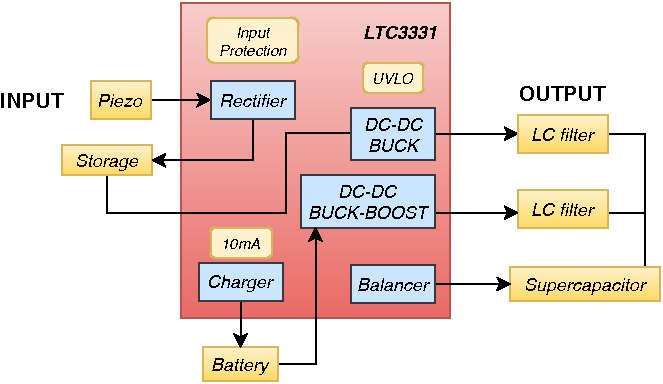
\includegraphics[scale=1.2]{LTC3331.pdf}
\caption{The diagram of \textit{LTC3331} based energy harvesting system}
\label{fig:ltc3331diagram}
\end{figure}
\par
The Table \ref{tab:ltc3331_params} lists the most important feature of the described integrated circuit. The input voltage range is broad enough to cover most of expected voltage values generated by piezoelectric harvesters. Moreover, the quiescent current of the device is very low, therefore the storage component is not excessively drained. The voltage drop of the integrated rectifier also helps to maintain high efficiency. 
\begin{table}[ht!]
\begin{tabular}{|l|c|}
\hline
\textbf{Parameter}	& \textbf{Value} 	\\ \hline
Model  				& LTC3331       \\ \hline
Manufacturer    	& Linear Technology	\\ \hline
Input operating range      &  2.7V to 19V 		\\ \hline
Quiescent current     &  950nA			\\ \hline
Output current        &  up to 50mA			\\ \hline
Selectable output voltages & from 1.8V to 5.0V \\ \hline
Input protection &  Shunt type (up to 25mA Pull-down)\\ \hline
Undervoltage lockout 	&  Yes (adjustable)		\\ \hline
Integrated rectifier 	&  Yes 		\\ \hline
Rectifier total drop 	&  800mV(at 10$\mu$A) 		\\ \hline
Battery charger max. current 	&  10mA 		\\ \hline
Balancer max. current 	&  10mA 		\\ \hline
\end{tabular}
\caption{Most important features taken from the manufacturer's datasheet \cite{ltc3331_params}}
\label{tab:ltc3331_params}
\end{table}
\par

\paragraph{Circuit design}
During the design process of the \textit{LTC3331} based circuit, the manufacturer's datasheet \cite{ltc3331_params} was a reference.
\par
Firstly, proper inductor has to be selected. The Buck converter is optimized for 22$\mu$H inductors. Nevertheless, it is possible to pick a higher value of inductance in order to increase the efficiency of the DC-DC Buck converter in high voltage applications \cite{ltc3331_params}. One should note that the DC resistance of the inductor has an impact on the overall efficiency of the converter. When it comes to the Buck-Boost converter, the manufacturer claims that the recommended inductance value is also 22$\mu$H. Please note that it is allowed to pick the another inductor, but the peak current of the inductor need to be adjusted by setting some of the integrated circuit's pins high or low - see the datasheet \cite{ltc3331_params}. For this occasion, a DIP switch has been installed. Eventually, the same inductor model has been selected for both converters. Its parameters are listed in the Table \ref{tab:ltc3331_inductor}.
\begin{table}[ht!]
\begin{tabular}{|c|c|c|c|c|}
\hline
\textbf{Manufacturer} & \textbf{Model} & \textbf{Inductance} & \textbf{Rated current} & \textbf{DC resistance}	\\ \hline
 Coilcraft & LPS4012-333 & 33$\mu$H & 0.46A & 0.825$\Omega$      \\ \hline
\end{tabular}
\caption{Inductor selected for the \textit{LTC3331}'s Buck and Buck-Boost converters \cite{ltc3331_inductor_params}}
\label{tab:ltc3331_inductor}
\end{table}
\par
The decision of using the larger value of inductance than the one recommended by the manufacturer is mostly due to the fact that the input voltage level of the Buck converter is currently unknown. As it was mentioned before, the higher inductance values increase the efficiency of the converter at higher input voltages, so the trade-off has been made. As to the Buck-Boost converter, it is possible to adjust the peak inductor current value, so there is no problem using higher inductances.
\par
When it comes to selection of suitable capacitors, the datasheet \cite{ltc3331_params} also served as a reference.
The input capacitor's recommended value depends on the input current generated by the piezoelectric element. By varying its value, it is possible to tune the harvester to maximize the amount of harvested energy. As a starting point, the input capacitor's value is set to 22$\mu$F, as this value has been proposed by the manufacturer in various reference designs.\par

When considering the output capacitor, the situation is almost the same, since the ripple current of the output capacitor depends on both the load and the amount of energy provided by the piezoelectric beam. One should remember to choose low inductance ceramic capacitors in SMD packages in order to minimize high frequency ripple introduced by the DC-DC converter \cite{companion}. At the prototyping stage, three 22$\mu$F ceramic capacitors has been connected in parallel, but this configuration could be a subject of change. Details in the Table \ref{tab:ltc3331_capacitors}.
\par

The purpose of the battery capacitor is to minimize the voltage droop when using the Buck-Boost converter \cite{ltc3331_params}. Having said that, it is important to place it relatively close to the integrated circuit in order to provide low impedance path for the converter's input \cite{companion}. The manufacturer's advice is to use 4.7$\mu$F or greater in order to maintain the performance \cite{ltc3331_inductor_params}. In this design, two general purpose  10$\mu$F tantalum capacitors in parallel has been chosen for this job, as they provide good compromise between capacitance and size. More details are included in the Table \ref{tab:ltc3331_capacitors}.

\begin{table}[ht!]
\begin{tabular}{|c|c|c|c|c|c|}
\hline
 \textbf{Type} & \textbf{Manufacturer} & \textbf{Model} & \textbf{Capacitance} & \textbf{Rated volt.} & \textbf{Count}	\\ \hline
Input & Würth Elektronik & 865060442002 & 22$\mu$F & 25V & 1      \\ \hline
Output & AVX & 12066C226MAT2A  & 22$\mu$F & 6.3V & 3      \\ \hline
Battery & AVX & TAJA106M010RNJ  & 10$\mu$F & 10V & 2      \\ \hline
\end{tabular}
\caption{Capacitors selected for the \textit{LTC3331} circuit \cite{ltc3588_capacitor_params}, \cite{x5r_params}, \cite{tantalum_params}}
\label{tab:ltc3331_capacitors}
\end{table}
\par

The layout of the designed circuit is presented in the Figure \ref{fig:ltc3331layout}. Similarly to the previous harvester, it is possible to change most of the settings of the integrated circuit by means of included DIP switches. This way, the evaluation of the \textit{LTC3331} 

\begin{figure}[ht!]
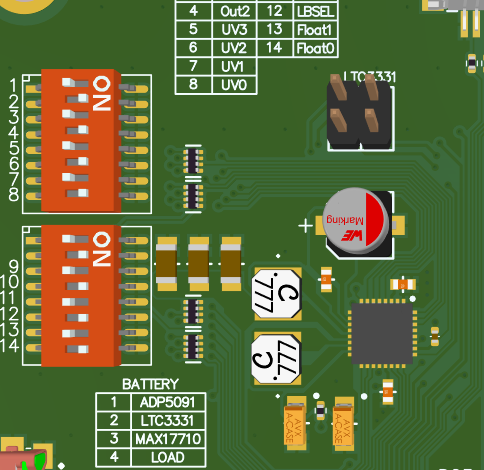
\includegraphics[scale=0.8]{ltc3331_layout.png}
\caption{The layout of \textit{LTC3331} based circuit}
\label{fig:ltc3331layout}
\end{figure}
\par

\subsubsection{ADP5091}

Another alternative for an integrated energy harvester is \textit{ADP5091} by \textit{Analog Devices}. This device is not dedicated exclusively for vibration energy harvesting applications. In case of piezo-based applications, it is necessary to provide an external voltage rectifier, as the described integrated circuit accepts only DC voltage at the input. One should note that \textit{ADP5091} incorporates a DC-DC boost converter and LDO, which is optimized for high efficiency at low output currents \cite{adp5091_params}.
\par

Figure \ref{fig:adp5091diagram} depicts the overall structure of the harvester. As mentioned before, the device is compatible with DC sources only. Having said that, it is necessary to perform input voltage conditioning by means of an external voltage rectifier. To further smooth the voltage, a storage capacitor is to be installed. Once the input voltage is rectified, the \textit{ADP5091} is able to perform a DC conversion in order to provide regulated output voltage. The described integrated circuit is combining two different voltage regulators, namely the LDO and the DC-DC Boost converter. In case of this design, only Boost converter would be used. Nevertheless, it is possible to select the hybrid operation mode, where both of regulators are used alternatively depending on the actual performance of the input power source\cite{adp5091_params}.

\begin{figure}[ht!]
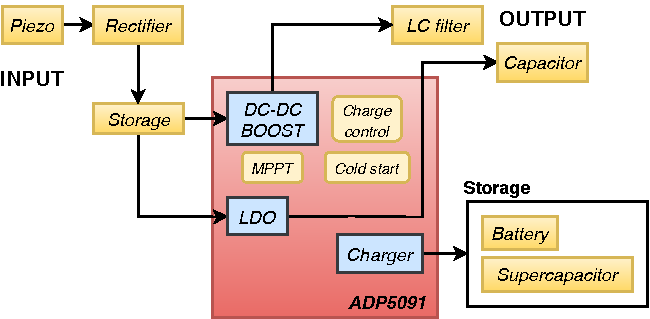
\includegraphics[scale=1.2]{adp5091.pdf}
\caption{The diagram of \textit{ADP5091} based energy harvesting system}
\label{fig:adp5091diagram}
\end{figure}

Due to the fact that the \textit{ADP5091} takes advantage of the DC-DC boost converter, this configuration is dedicated for low output voltage piezoelectric generators. Table \ref{tab:adp5091_params} lists the most important parameters of the device.
\par

\begin{table}[ht!]
\begin{tabular}{|l|c|}
\hline
\textbf{Parameter}	& \textbf{Value} 	\\ \hline
Model  				& ADP5091       \\ \hline
Manufacturer    	& Analog Devices	\\ \hline
Input operating range      &  0.08V to 3.3V  \\ \hline
Quiescent current     &  510nA (typical)		\\ \hline
Output current        &  up to 150mA			\\ \hline
Selectable output voltages & from 1.5V to 3.6V\\ \hline
Integrated rectifier 	&  No 		\\ \hline
Fast Cold Start threshold voltage 	&  380mV 	\\ \hline
Optional back-up 	&  Yes (primary battery) 	\\ \hline
MPPT 	&  Yes 		\\ \hline
\end{tabular}
\caption{Most important features taken from the manufacturer's datasheet \cite{adp5091_params}}
\label{tab:adp5091_params}
\end{table}
One should note relatively low input voltage operating range. In order to face this problem, it may be required to use a relatively high input capacitance that would impose more load on the piezoelectric generator, therefore reducing its output voltage \cite{EnHv2}. The \textit{ADP5091} has remarkably low quiescent current, what is one of the most important aspects in energy harvesting applications. In addition to that, the manufacturer claims it provides an MPPT feature. The input voltage threshold is as low as 380mV, what makes it possible to maximize the amount of harvested energy. 
\par

\paragraph{Circuit design}
The selected inductor should have saturation current at least 30\% higher than the peak inductor current (which might be as high as 300mA) and relatively low DC resistance in order to maintain high efficiency \cite{adp5091_params}. The converter is optimized for 22$\mu$H inductors. By combining all mentioned parameters, the inductor listed in the Table \ref{tab:adp5091_inductor} has been selected.
\begin{table}[ht!]
\begin{tabular}{|c|c|c|c|c|}
\hline
\textbf{Manufacturer} & \textbf{Model} & \textbf{Inductance} & \textbf{Rated current} & \textbf{DC resistance}	\\ \hline
 Würth Elektronik & 744042220 & 22$\mu$H & 0.88A & 0.3$\Omega$      \\ \hline

\end{tabular}
\caption{Inductor selected for the \textit{ADP5091} circuit \cite{adp5091_inductor_params}}
\label{tab:adp5091_inductor}
\end{table}
\par

Input capacitor is utilized to store energy captured from the piezoelectric beam. Its value recommended by the manufacturer is at least 10$\mu$F, but larger values may be beneficial in case when an additional primary battery is used \cite{adp5091_params}. In case of this design, the minimum recommended value would be a way to go.
\par
The output capacitor is used to smooth the output voltage of the switching regulator. Even though, the minimum recommended value is 4.7$\mu$F, it would be extended to 22$\mu$ to further smooth the output voltage. There are a few more capacitor required by the integrated circuit to operate properly, but all of them would be picked according to the manufacturer's recommendations. Please see Table \ref{tab:adp5091_capacitors} for details regarding input and output capacitors.

\begin{table}[ht!]
\begin{tabular}{|c|c|c|c|c|c|}
\hline
 \textbf{Type} & \textbf{Manufacturer} & \textbf{Model} & \textbf{Capacitance} & \textbf{Rated voltage} & \textbf{Count}	\\ \hline
Input & AVX & TAJA106M010RNJ  & 10$\mu$F & 10V & 1      \\ \hline
Output & AVX & 12066C226MAT2A  & 22$\mu$F & 6.3V & 1      \\ \hline
\end{tabular}
\caption{Capacitors selected for the \textit{ADP5091} circuit \cite{x5r_params}, \cite{tantalum_params}}
\label{tab:adp5091_capacitors}
\end{table}
\par

The last important aspect to mention is related to the full bridge rectifier's diodes. Owing to the fact that the forward voltage drop of these components has a huge impact on the overall efficiency of the power management circuit, one should select diodes suitable for this application. The designer's choice is placed in the Table \ref{tab:adp5091_diodes}. Please note that the forward voltage drop of these diodes conducting low current might be way lower than 200mV \cite{diodes_params}.
\begin{table}[ht!]
\begin{tabular}{|c|c|c|c|}
\hline
\textbf{Manufacturer} & \textbf{Model} & \textbf{Forward voltage ($I_f=500mA$)} & \textbf{Forward Current}\\ \hline
 Nexperia & PMEG4005EJ & 0.42V & 0.5A      \\ \hline

\end{tabular}
\caption{Rectifier diodes selected for the \textit{ADP5091} circuit \cite{diodes_params}}
\label{tab:adp5091_diodes}
\end{table}
\par

The layout of the \textit{ADP5091}-based circuit in presented in the figure \ref{fig:adp5091layout}. One should note a DIP switch that makes it easy to change some of the inegrated circuit's settings. This feature is particularly useful during the circuit evaluation process.
\begin{figure}[ht!]
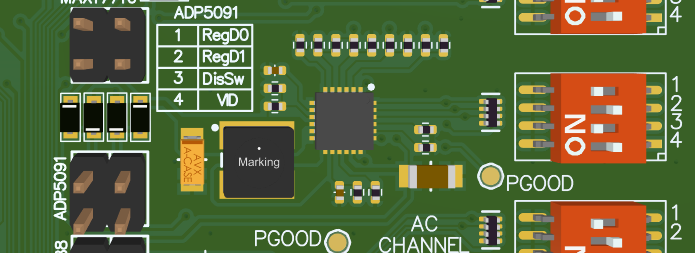
\includegraphics[scale=0.8]{adp5091_layout.png}
\caption{The layout of \textit{ADP5091} based circuit}
\label{fig:adp5091layout}
\end{figure}
\par
\subsubsection{MAX17710}
The last of selected devices is \textit{MAX17710} by \textit{Maxim Integrated}. It is a complete system for charging and protecting small storage devices \cite{max17710_params}. The manufacturer claims that the device can handle generators with output power levels as low as 1$\mu$W. The output of the regulator is based on the very low quiescent current LDO, which also incorporates overdischarge protection of the battery.
\par

The figure \ref{fig:max17710diagram} presents the most important features of the described device. In case of this design, only the low-dropout regulator would utilized according to the manufacturer's recommendations \cite{max17710_params}, thus the DC-DC Boost converter is not mentioned in the diagram. The input part looks similar to the one described in the section regarding \textit{ADP5091}. Due to the fact that \textit{MAX17710} requires DC voltage at the input, the full bridge rectifier  along with the storage capacitor are installed. The input power is used to charge the storage component, which could be both a rechargeable battery or a supercapacitor. Once there is a sufficient amount of charge stored, the LDO is able to source the output. The output voltage level can be adjusted according to the user's needs. In case the input charging voltage is higher than the allowed storage element voltage, the entire power is sourced to the LDO. Moreover,the device features the input overvoltage protection formed by a shunt diode. The storage component is also protected against over-discharge conditions \cite{max17710_params}. Some of the most important features  of the device are once again summarized in the Table \ref{tab:max17710_params}.

\begin{table}[ht!]
\begin{tabular}{|l|c|}
\hline
\textbf{Parameter}	& \textbf{Value} 	\\ \hline
Model  				& MAX17710       \\ \hline
Manufacturer    	& Maxim Integrated	\\ \hline
Maximum Input Voltage      &  5.3V  \\ \hline
Quiescent current     &  626nA (during charging)\\ \hline
Output current        &  up to 75mA			\\ \hline
Selectable output voltages & from 1.8V to 3.3V\\ \hline
Integrated rectifier 	&  No 		\\ \hline
Over-voltage protection clamping current & up to 50mA \\ \hline
Maximum Charging Current 	&  100mA 	\\ \hline
\end{tabular}
\caption{Most important features taken from the manufacturer's datasheet \cite{max17710_params}}
\label{tab:max17710_params}
\end{table}
\par

Similarly to other described integrated circuits, \textit{MAX17710} has significantly low quiescent current, what allows for energy harvesting using power sources with output capabilities as low as 1$\mu$W. Another interesting feature is the shunt input protection capable of clamping up to 50mA.
\par

\paragraph{Circuit design}

\begin{figure}[ht!]
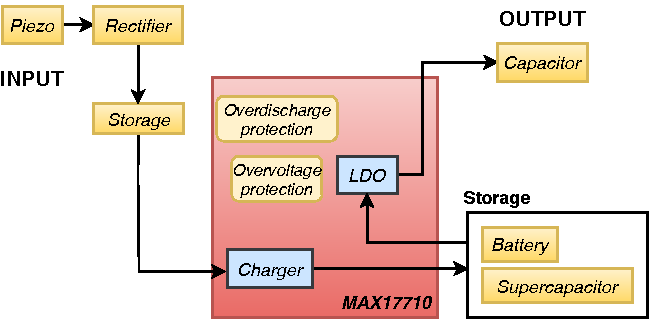
\includegraphics[scale=1.2]{MAX17710.pdf}
\caption{The diagram of \textit{MAX17710} based energy harvesting system}
\label{fig:max17710diagram}
\end{figure}

\par

\begin{figure}[ht!]
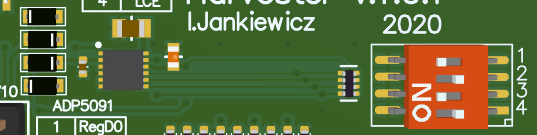
\includegraphics[scale=1.0]{max17710_layout.png}
\caption{The layout of \textit{MAX17710} based circuit}
\label{fig:max17710layout}
\end{figure}

\par

\begin{figure}[ht!]
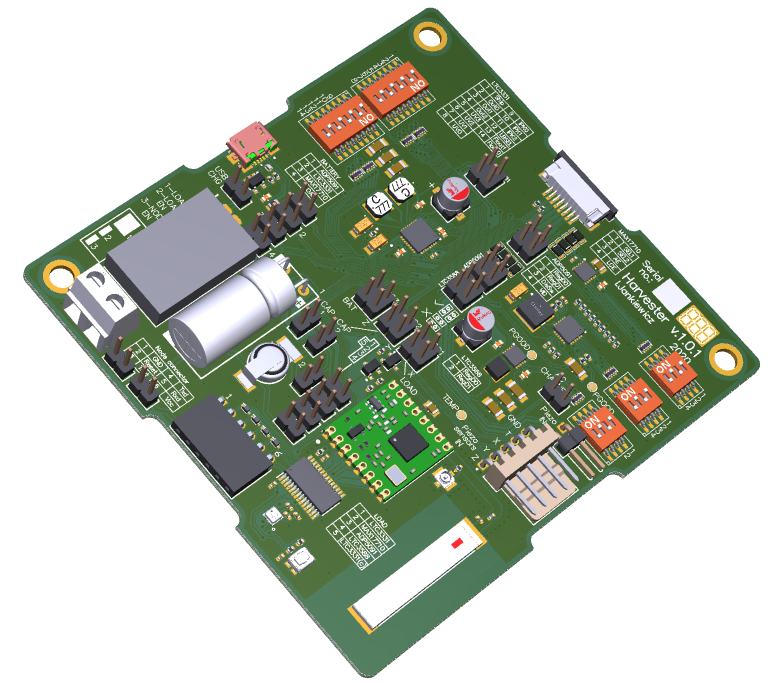
\includegraphics[scale=0.75]{harvester2.png}
\caption{Harvester board 3D model}
\label{fig:harvester3d}
\end{figure}



\clearpage

\printbibliography

%\bibliography{bibliography} 
%\bibliographystyle{ieeetr}


\end{document}
